\documentclass[fleqn]{jbook}
\usepackage{physpub}

\begin{document}

\begin{question}{専攻 問題8}{}

核酸やタンパク質分子は、ヌクレオチドやアミノ酸を骨格要素とする
直鎖状高分子である。図は$(n+1)$個の骨格要素からなる直鎖状高分子の
コンフィギュレーションを描いたものである。骨格要素は円で示されている。
$i$番目の骨格要素の位置ベクトルを$\vec{r}_i$、$i-1$番目と$i$番目
の骨格要素をつなぐ結合ベクトルを$\vec{b}_i$とする。
結合ベクトルの大きさはすべて$b$である。以下の設問に答えよ。

\begin{center}
  \mbox{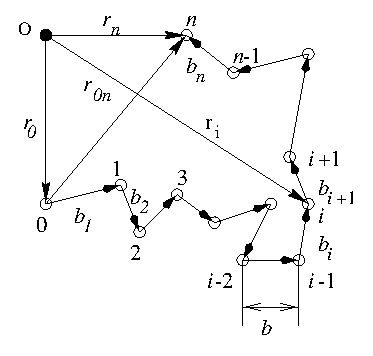
\includegraphics[clip]{1994phy8-1.eps}}
\end{center}

\begin{subquestions}
\SubQuestion
  結合ベクトルの向きが互いに完全にランダムである鎖を自由連結鎖という。
自由連結鎖について、$\vec{b}_i\cdot\vec{b}_j$の期待値である
$<\vec{b}_i\cdot\vec{b}_j>$を求めよ。

\SubQuestion
  鎖の両末端を結ぶベクトルを$\vec{r}_{0n}=\vec{r}_n-\vec{r}_0$
とする。自由連結鎖の両末端距離の2乗の平均$<{\vec{r}_{0n}}^2>$を求めよ。

\SubQuestion
  鎖の広がりを表す回転半径$R_G$は、各骨格要素と鎖の重心との
距離の2乗の平均の平方根で定義される。$R_G$が、
\[R_G=\frac{1}{n+1}\left(\sum_{0\leq i<j\leq n}
\left\langle\left(\vec{r}_i-\vec{r_j}\right)^2\right\rangle\right)^{1/2}\]
で与えられることを用いて、$n\rightarrow \infty$での$R_G$と
$<{\vec{r}_{0n}}^2>$との関係を示せ。

\SubQuestion
  大腸菌ゲノムの大きさは、$5\times10^6$塩基対である。ゲノムDNA
分子を塩基対を骨格要素とする自由連結鎖とみなし、
$R_G$および$<\vec{r}_{0n}^2>^{1/2}$を有効数字1桁で求めよ。
なお、DNA2重らせんの塩基対間距離は0.3nmである。

\SubQuestion
   実在するDNA分子は、隣り合う塩基対同士の連絡が自由でないので、
塩基対を骨格要素とする自由連結鎖とみなすことはできない。しかし、
実在するDNA分子の十分に離れた塩基対どうしはあたかも自由に連結
されているかのようにふるまう。したがって、長さが$n$塩基対の実在DNA分子は、
$n$が十分に大きいとき、$n/a$個の仮想的な骨格要素を長さ$ab$
の仮想的な結合で連結した自由連結鎖とみなすことができる。
実験によると、生理的条件では$a=500$である。大腸菌のゲノムDNA分子を
仮想的な骨格要素からなる自由連結鎖と考え、$R_G$および
$<\vec{r}_{0n}^2>^{1/2}$を有効数字1桁で求めよ。

\SubQuestion
  大腸菌の大きさは約$\rm 1\mu m$である。この大きさと設問{\bf 5}で得られた
そのゲノムDNA分子の大きさとを比較し、両者の違いの生物学的意味について述べよ。

\SubQuestion
  直鎖高分子の溶液中での大きさを測定する実験方法を二つあげ、
その原理と方法を具体的に述べよ。

\end{subquestions}
\end{question}
\begin{answer}{専攻 問題8}{}

\begin{subanswers}
\SubAnswer

%  \[ \Mean{\vec{b}_i \cdot \vec{b}_j}%
%     \geq b^2\Dint{0}{\pi}{\d{\theta}}\cos\theta = 0 \]

   \[ \Mean{\vec{b}_i \cdot \vec{b}_j}
       = \delta_{i j}\Mean{\vec{b}^2}+
        \delta_{i\neq j}\Mean{\vec{b_i}}\Mean{\vec{b_j}} 
      =b^2\delta_{ij} \]

   (\Naze $i\neq j$のとき、ランダムに向きが動くので、$\vec{b_i}$と
        $\vec{b_j}$の相関がなく、freeである。) 

\SubAnswer

  $\vec{r_{0n}}=\sum_{i=0}^{n}\vec{b_i}$より、
   \[ \Mean{\vec{r_{0n}}^2}
      =\sum_{i,j}\Mean{\vec{b_i}\cdot \vec{b_j}}
      =\sum_{i,j} \delta_{i j}b^2 
      =nb^2 
   \]
  
%  \[ \Mean{\vec{r{}}_{0n}^2}%
%     = \sum_{i,j} \Mean{\vec{b}_i \cdot \vec{b}_j}%
%     = \sum_{i} \Mean{\vec{b}_i \cdot \vec{b}_i} = nb^2 \]
%
%  ただし、設問{\bf 1}の結果によって$i\neq j$の項が消えることを
%  利用した。

\SubAnswer

   $\vec{r_j}-\vec{r_i}=\ds{\sum_{k=i+1}^j}\vec{b_k}$(但し$j>i$)なので、
     \[ \Mean{(\vec{r_i}-\vec{r_j})^2}=
         \Mean{\sum_{k=i+1}^{j}\vec{b_k}\cdot \sum_{l=i+1}^{j}\vec{b_l}}
         =\sum_{k,l=i+1}^{j}\delta_{k l} b^2 =|j-i|b^2 \]
     \[ \Yueni \sum_{0\leq i< j \leq n}\Mean{(\vec{r_i}-\vec{r_j})^2}
        =\sum_{0\leq i<j \leq n} |j-i|b^2 =\frac{1}{6}n(n+1)(n+2)b^2 \]
    となるから、$n\rightarrow \infty$で、
    \[ R_G=\sqrt{\frac{1}{6}nb^2 \frac{(n+1)(n+2)}{(n+1)^2}}
       \simeq \sqrt{\frac{1}{6}nb^2}=\sqrt{\frac{1}{6}\Mean{\vec{r_{0n}}^2}}\] 

%  $\vec{r}_i - \vec{r}_j$ は分散が $|i-j| b^2$ の Gauss 分布を
%  しているので、
%
%  \[ \Mean{( \vec{r}_i - \vec{r}_j )^2} = |i-j| b^2 \]
%
%  であるから、
%
%  \[ R_G^2=\frac{1}{2(n+1)^2}\sum^{n}_{i=0}\sum^{n}_{j=0}|i-j|b^{2}\]
%
%  となる。ここで、$n \rightarrow \infty $ では和を積分に置き換えても
%  よく、
%
%  \[ R_G^2 \approx \frac{b^2}{2n^2} \Dint{0}{n}{\d{i}}%
%                \Dint{0}{n}{\d{j}} |i-j| = \frac{1}{6}nb^2 \]
%
%  となるので、$ R_G^2 = \frac{1}{6} \Mean{\vec{r{}}_{0n}^2}$ となる。


\SubAnswer
  $n=5\Keta{6}$、$b=3\Keta{-10}\Unit{m}$
  よって$nb^2=45\Keta{-14}\Unit{m^2}$より、
%
  \[ \Mean{\vec{r{}}_{0n}^2}^{1/2}%
     = 7\Keta{-7}[\Unit{m}] = 0.7 [\Unit{\mu m}] \]
  \[ R_G \simeq \sqrt{\frac{1}{6}}\Mean{\vec{r{}}_{0n}^2}^{1/2}
               \simeq 0.3[\Unit{\mu m}] \]
%

\SubAnswer

  設問{\bf 4}において、$n'=n/a=1\Keta{4}$、$b'=ab=1.5\Keta{-7}\Unit{m}$
  とおき直して計算。
%
  \[ n'b^{\prime 2} = 2.25\Keta{-10}\Unit{m^2} \]
%
  よって、
%
  \[ \Mean{\vec{r{}}_{0n}^2}^{1/2}%
     = 1.5\Keta{-5}[\Unit{m}] = 15[\Unit{\mu m}] \]
  \[ \Yueni R_G =6 [\Unit{\mu m}] \] 
%
\SubAnswer
%  大腸菌DNAを自由連結鎖とみなすと、大腸菌に入り切らない。
%  すなわち、大腸菌DNAは大腸菌内では自由鎖ではなく、
%  何らかの力が働くことによってコンパクトに折り畳まれて
%  いることが考えられる。
   大腸菌の中で、ゲノムDNAはランダムコイル状態にあるのではなく、何らか
   の機構により、コンパクトに折り畳まれていると考えられる。コンパ
   クトな形に定まっていることにより、表面積を小さくし、紫外線など
   外界の危険をなるべく避けることに成功していると考えられる。


\SubAnswer
  {\bf [ゲルろ過法]}\\
  凹凸のついたビーズをカラムに詰め、その中に溶液を
  流す。大きさの大きいものほど早く落ちてくるので、
  それによって分子の大きさを知ることができる。\\
  {\bf [拡散係数を測定する]}\\
  拡散係数が分子の大きさの関数になっている
  ので、拡散の度合を光散乱で測定すればそれより分子の
  おおよその大きさが計算できる。
  
  そのほか、粘性の測定・流動複屈折(屈折率の方向依存性の測定)・光散乱
  の利用が考えられる。
\end{subanswers}
\end{answer}


\end{document}
